\documentclass[12pt]{article}
\usepackage{fancyhdr}
\usepackage{color}
\usepackage{multicol}
\usepackage{fancyvrb}
\usepackage{enumitem}
\usepackage{graphicx}
\usepackage{sectsty}
\usepackage{amsmath}
\usepackage{amssymb}
\usepackage{hyperref}
\usepackage{array}
\newcommand{\sectionbreak}{\clearpage}

\usepackage{tikz}
\usepackage{tkz-euclide}
\usetkzobj{all}

\allsectionsfont{\centering}

\usepackage{draftwatermark}
	\SetWatermarkText{\copyright wolf-math.com}
	\SetWatermarkScale{4}
	\SetWatermarkLightness{1}

\usepackage[margin=1in, headsep=0pt]{geometry}
\setlength{\parindent}{0cm}
\pagestyle{empty}

\begin{document}

Mr. Wolf  \\ wolf-math.com

\section*{Law of Sines \& Law of Cosines}

\subsection*{Goals}

\textbf{I will be able to} use the Law of Sines to solve \textbf{Angle-Angle-Side}, \textbf{Angle-Side-Angle}, and \textbf{Side-Side-Angle} triangles for their unknown sides.\\

\textbf{I will be able to} determine if there is 1 solution, 2 solutions, or no solutions to a triangle.\\

\textbf{I will be able to} use the Law of Cosines to solve \textbf{Side-Angle-Side} and \textbf{Side-Side-Side} triangles.\\

\textbf{I will be able to} determine the correct law to solve any triangle.\\

\textbf{I will be able to} use both the Law of Sines and the Law of Cosines in the same triangle to solve that triangle.\\

\subsection*{Standards}

\textbf{Similarity, Right Triangles, and Trigonometry \hfill G-SRT}\\

Apply trigonometry to general triangles\\

11. (+) Understand and apply the Law of Sines and the Law of Cosines to find
unknown measurements in right and non-right triangles (e.g., surveying
problems, resultant forces).\\

\subsection*{Connections}

\textbf{Before} we learned about how trigonometry is used to solve for right triangles. \\

\textbf{Now} we are learning how trigonometry is applied to any triangle.\\

\textbf{After} we will be learning the unit circle and the way trigonometry is applied to the coordinate plane. This is called \textit{analytic geometry}.\\

\let\stdsection\section
\renewcommand\section{\newpage\stdsection}

\section*{The Law of Sines}

The \textbf{Law of Sines} helps us solve for \textbf{non}-right triangles. It is simply a proportion that we need to solve for.\\

$$\frac{\sin(A)}{a}=\frac{\sin(B)}{b}=\frac{\sin(C)}{c}$$

or 

$$\frac{a}{\sin(A)}=\frac{b}{\sin(B)}=\frac{c}{\sin(C)}$$

\begin{center}
\includegraphics[scale=1]{triangle01.jpg}
\end{center}


\begin{multicols}{2}
Capital letters always represent \textit{angles}. \\
Lowercase letters always represent \textit{sides}.\\

\columnbreak

Angle $A$ is always opposite side $a$.\\
Angle $B$ is always opposite side $b$.\\
Angle $C$ is always opposite side $c$.\\

\end{multicols}

\subsection*{Solving for a Side: Side - Angle - Side}

\begin{center}
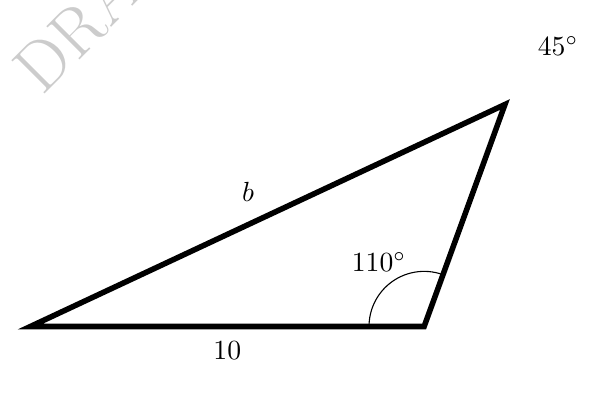
\begin{tikzpicture}

	\coordinate (a) at (0,0);
	\coordinate (b) at (5,0);
	\coordinate (c) at (6.02606043,2.819077826);
	\draw[line width=2pt] (a) -- (b) -- (c) -- cycle;
	
	\tkzMarkAngle[size=.7](c,b,a)
	\tkzLabelAngle[pos=1](c,b,a){$110^\circ$}
	\tkzLabelSegment[below = 2pt](a,b){$10$}
%	\tkzLabelSegment[right = 2pt](b,c){$6$}
	\tkzLabelSegment[above left =2pt](c,a){$b$}
%	\tkzLabelAngle(c,a,b){$A$}
	\tkzLabelAngle(b,c,a){$45^\circ$}

\end{tikzpicture}
\end{center}

Since we're solving for a side, put the unknown side on the top-left fraction, then solve for $b$.\\

$$\frac{b}{\sin(110)}=\frac{10}{\sin(45)}$$\\

$$b=\frac{10\sin(110)}{\sin(45)}\approx 13.3$$

\subsection*{Solving for an Angle: Side - Side - Angle}

\begin{center}
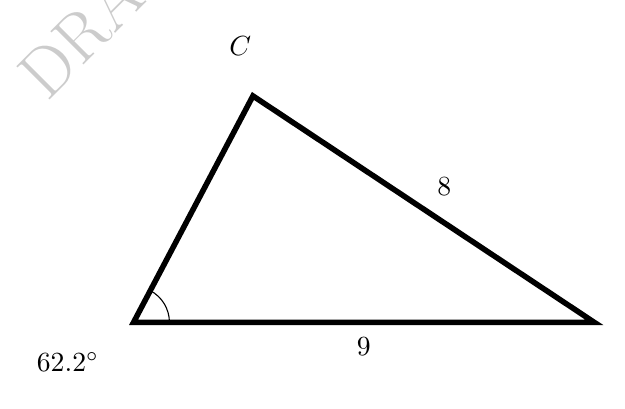
\begin{tikzpicture}[scale=.65]
	
	\coordinate (a) at (0,0);
	\coordinate (b) at (9,0);
	\coordinate (c) at (2.331933202,4.422904876);
	\draw[line width =2 pt] (a) -- (b) -- (c) -- cycle;
	
	\tkzMarkAngle[size=.7](b,a,c)
	\tkzLabelAngle[pos=1.5](c,a,b){$62.2^\circ$}
	\tkzLabelSegment[below = 2pt](a,b){9}
%	\tkzLabelSegment[above left = 2pt](c,a){5}
	\tkzLabelSegment[above right = 2pt](b,c){8}
	\tkzLabelAngle(b,c,a){$C$}
%	\tkzLabelAngle(a,b,c){$B$}

	
\end{tikzpicture}
\end{center}

Since we're solving for an angle we must use an \textit{inverse sine} to finish the problem. Just like above, we put the unknown in the top left of the fraction.\\

$$\frac{\sin(C)}{9}=\frac{\sin(62.2)}{8}$$\\

$$\sin(C)=\frac{9\sin(62.2)}{8}$$\\

$$C=\sin^{-1}\left(\frac{9\sin(62.2)}{8}\right)\approx84.36$$

\section*{Law of Sines Proof}

\begin{center}
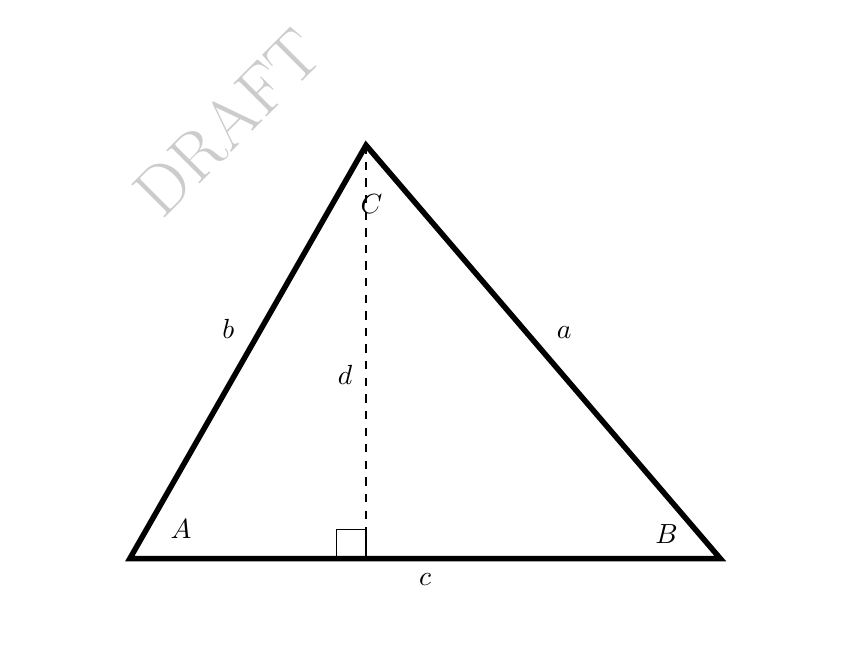
\begin{tikzpicture}[scale=1.5]

	\coordinate (a) at (0,0);
	\coordinate (b) at (5,0);
	\coordinate (c) at (2,3.5);
	\coordinate (d) at (2,0);
	\draw[line width=2pt] (a) -- (b) -- (c) -- cycle;
	\draw[dashed](c) -- (d);
	
	\tkzLabelSegment[below = 2pt](a,b){$c$}
	\tkzLabelAngle[pos=-.5](b,c,a){$C$}
	\tkzLabelSegment[above right=2pt](b,c){$a$}
	\tkzLabelAngle[pos=-.5](c,a,b){$A$}
	\tkzLabelSegment[above left=2pt](c,a){$b$}
	\tkzLabelAngle[pos=-.5](a,b,c){$B$}
	\tkzLabelSegment[below left=2pt](c,d){$d$}
	\tkzMarkRightAngle(a,d,c)


\end{tikzpicture}
\end{center}

\begin{center}
\begin{tabular}{c | c}

$\sin(A)=\frac{d}{b}$ &  $\sin(B)=\frac{d}{a}$ \\ 

 & \\

$d=b\sin(A)$ &  $d=a\sin(B)$ \\ 


\end{tabular}


\vspace{12pt}

 $b\sin(A)=a\sin(B)$  \\ \vspace{12pt}

$\frac{b}{\sin(B)}=\frac{a}{\sin(A)}$ \\ \vspace{12pt}
\end{center}


\section*{Law of Cosines}

The \textbf{Law of Cosines} is the Pythagorean Theorem of all triangles, not just right triangles.

\begin{center}

$a^2=b^2+c^2-2bc\cos(A)$\\

$b^2=a^2+c^2-2ac\cos(B)$\\

$c^2=a^2+b^2-2ab\cos(C)$\\

\end{center}

Which one of these you use depends on what you're trying to solve for.\\

\hrulefill

\subsection*{Solving for a side: Side-Angle-Side}



\textbf{4 - step process}

\begin{enumerate}

\item Label all of your points -- This keeps them straight in your head.\\

\item Plug the pieces into the proper places. $b^2=a^2+c^2-2ac\cos(B)$\\

\item Evaluate.\\

\item Take square root.\\
\end{enumerate}

\begin{center}
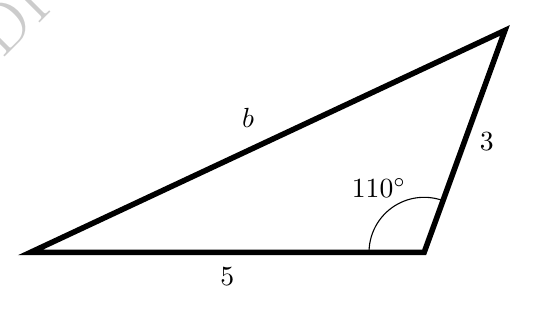
\begin{tikzpicture}

	\coordinate (a) at (0,0);
	\coordinate (b) at (5,0);
	\coordinate (c) at (6.02606043,2.819077826);
	\draw[line width=2pt] (a) -- (b) -- (c) -- cycle;
	
	\tkzMarkAngle[size=.7](c,b,a)
	\tkzLabelAngle[pos=1](c,b,a){$110^\circ$}
	\tkzLabelSegment[below = 2pt](a,b){$5$}
	\tkzLabelSegment[right = 2pt](b,c){$3$}
	\tkzLabelSegment[above left =2pt](c,a){$b$}
%	\tkzLabelAngle(c,a,b){$A$}
%	\tkzLabelAngle(b,c,a){$C$}
\end{tikzpicture}
\end{center}

\[
\begin{array}{c c c l }
\text{Step 2:}	& b^2 	& = 		& 5^2+3^2-2(5)(3)\cos(110) 	\\		\vspace{12pt}
				& b^2 	& = 		& 25+9-30\cos(110) 			 \\ 	\vspace{12pt}
\text{Step 3:}	& b^2 	& \approx 	& 44.2606043				 \\	%\vspace{12pt}
\text{Step 4:}	& b 	& = 		& \sqrt{44.2606043} \approx 6.5  \\
\end{array}
\]



\subsection*{Solving for an angle: Side - Side - Side}



To solve for $A$, $a^2=b^2+c^2-2bc\cos(A)$ could be used. Instead we will use an alternate version of the same equation. This is the same equation, except that we're looking to solve and angle, so it's automatically solved for the $\cos(x)$. You can still use the above Law of Cosines to set up and solve.\\

$$\cos(A)=\frac{a^2-b^2-c^2}{-2bc}$$

$$\cos(B)=\frac{b^2-a^2-c^2}{-2ac}$$

$$\cos(C)=\frac{c^2-a^2-b^2}{-2ab}$$\\

\textbf{4 - step process to solve for an angle}

\begin{enumerate}

\item Label all of your sides and angles.\\

\item Plug your values into the equation.\\

\item Evaluate.\\

\item Calculate $\cos^{-1}$ to determine the angle.\\
\end{enumerate}

%\cos(A)=\frac{a^2-b^2-c^2}{-2bc}

\begin{center}
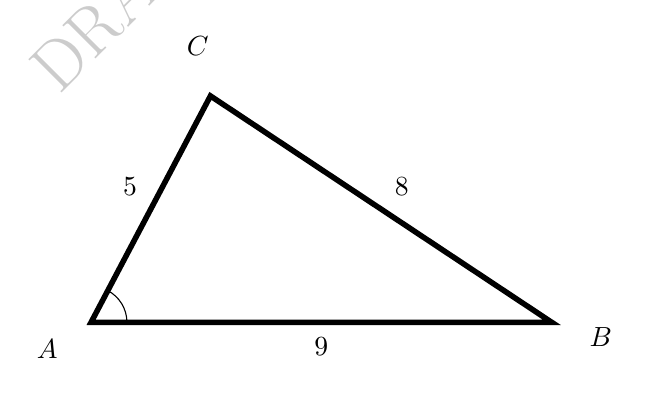
\begin{tikzpicture}[scale=.65]
	
	\coordinate (a) at (0,0);
	\coordinate (b) at (9,0);
	\coordinate (c) at (2.331933202,4.422904876);
	\draw[line width =2 pt] (a) -- (b) -- (c) -- cycle;
	
	\tkzMarkAngle[size=.7](b,a,c)
	\tkzLabelAngle(c,a,b){$A$}
	\tkzLabelSegment[below = 2pt](a,b){9}
	\tkzLabelSegment[above left = 2pt](c,a){5}
	\tkzLabelSegment[above right = 2pt](b,c){8}
	\tkzLabelAngle(b,c,a){$C$}
	\tkzLabelAngle(a,b,c){$B$}

	
\end{tikzpicture}
\end{center}

\[
\begin{array}{c c c l }
\text{Step 2:}	& \cos(A) 	& = 		& \frac{8^2-5^2-9^2}{-2(5)(9)} 	\\		\vspace{12pt}
				& \cos(A) 	& = 		& \frac{-42}{-90} 			 \\ 	\vspace{12pt}
\text{Step 3:}	& \cos(A) 	& \approx 	& .466				 \\	%\vspace{12pt}
\text{Step 4:}	& A		 	& = 		& \cos^{-1}(.466) \approx 62  \\
\end{array}
\]

\section*{Law of Cosines Proof}

\begin{center}
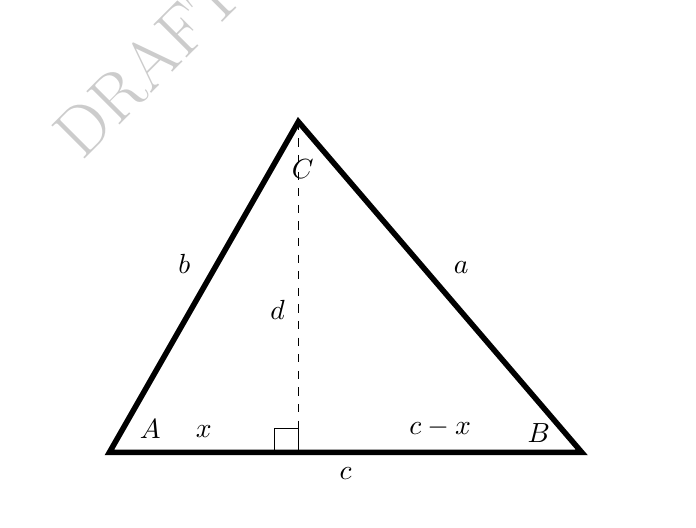
\begin{tikzpicture}[scale=1.2]

	\coordinate (a) at (0,0);
	\coordinate (b) at (5,0);
	\coordinate (c) at (2,3.5);
	\coordinate (d) at (2,0);
	\draw[line width=2pt] (a) -- (b) -- (c) -- cycle;
	\draw[dashed](c) -- (d);
	
	\tkzLabelSegment[below = 2pt](a,b){$c$}
	\tkzLabelAngle[pos=-.5](b,c,a){$C$}
	\tkzLabelSegment[above right=2pt](b,c){$a$}
	\tkzLabelAngle[pos=-.5](c,a,b){$A$}
	\tkzLabelSegment[above left=2pt](c,a){$b$}
	\tkzLabelAngle[pos=-.5](a,b,c){$B$}
	\tkzLabelSegment[below left=2pt](c,d){$d$}
	\tkzMarkRightAngle(a,d,c)
	
	\tkzLabelSegment[above = 2pt](a,d){$x$}
	
	\tkzLabelSegment[above = 2pt](d,b){$c-x$}


\end{tikzpicture}
\end{center}



$$\cos(A)=\frac{x}{b} \Longrightarrow x=b\cos(A)$$

$$h^2=b^2-x^2 \hspace*{1in} h^2=a^2-(c-x)^2$$\\

set $h$ equal to itself

$$b^2-x^2=a^2-(c-x)^2$$\\

expand the square of a binomial

$$b^2-x^2=a^2-c^2+2cx-x^2$$\\

$x^2$ cancells out

$$b^2=a^2-c^2+2cx$$\\

$x=b\cos(A)$ from above

$$b^2=a^2-c^2+2cb\cos(A)$$\\

solving for $a^2$

$$a^2=b^2+c^2-2cb\cos(A)$$







\section*{Law of Sines vs. Cosines}

Which law do you use? The law of sines is used for side-side-angle and side-angle-side, while the law of cosines is used for s

\begin{multicols}{2}
\setlength{\columnsep}{1.5cm}
\setlength{\columnseprule}{2pt}


\subsection*{Law of Sines}

\textbf{2 sides, 1 opposite angle}\\

\begin{center}
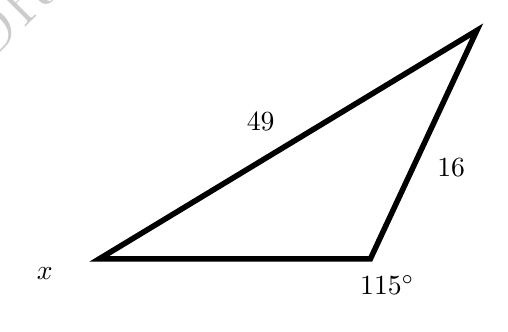
\begin{tikzpicture}[scale=.4]

	\coordinate (a) at (0,0);
	\coordinate (b) at (8.605,0);
	\coordinate (c) at (11.985,7.25);
	\draw[line width = 2pt] (a) -- (b) -- (c) -- cycle;
	
	\tkzLabelSegment[above left = 2pt](a,c){$49$}
	\tkzLabelSegment[below right = 2pt](b,c){$16$}
	\tkzLabelAngle[pos=1.8](c,a,b){$x$}
	\tkzLabelAngle(a,b,c){$115^\circ$}	

\end{tikzpicture}
\end{center}

\vspace{12pt}

\textbf{2 angles, 1 opposite side}\\

\begin{center}
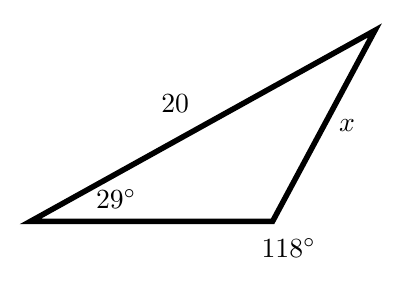
\begin{tikzpicture}[scale=.25]

	\coordinate (a) at (0,0);
	\coordinate (b) at (12.3,0);
	\coordinate (c) at (17.5,9.7);
	\draw[line width=2pt] (a) -- (b) -- (c) -- cycle;
	
%	\tkzMarkAngle(b,a,c)
	\tkzLabelAngle[pos=4.5](b,a,c){$29^\circ$}
	\tkzLabelAngle[pos=1.6](a,b,c){$118^\circ$}
	\tkzLabelSegment[right=2pt](b,c){$x$}
	\tkzLabelSegment[above left = 2pt](c,a){20}

\end{tikzpicture}
\end{center}


\columnbreak

\subsection*{Law of Cosines}

\begin{center}

\textbf{2 sides, 1 angle inbetween}\\

\vspace{12pt}

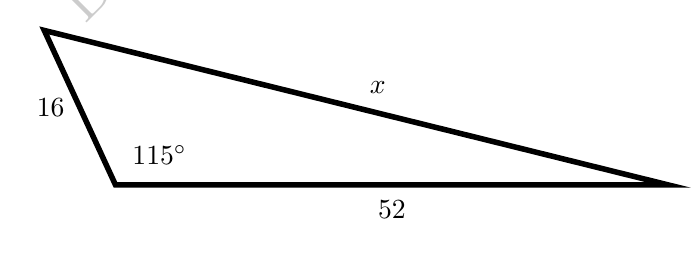
\begin{tikzpicture}[scale=.135]

	\coordinate (a) at (6.7,0);
	\coordinate (b) at (58.7,0);
	\coordinate (c) at (0,14.533);
	\draw[line width = 2pt] (a) -- (b) -- (c) -- cycle;
	
	\tkzLabelSegment[left=2pt](c,a){$16$}
	\tkzLabelSegment[above right = 2pt](b,c){$x$}
	\tkzLabelSegment[below = 2pt](a,b){$52$}
	\tkzLabelAngle[above right =.75pt](b,a,c){$115^\circ$}
	

\end{tikzpicture}


\vspace{1in}

\textbf{3 sides, no angles}


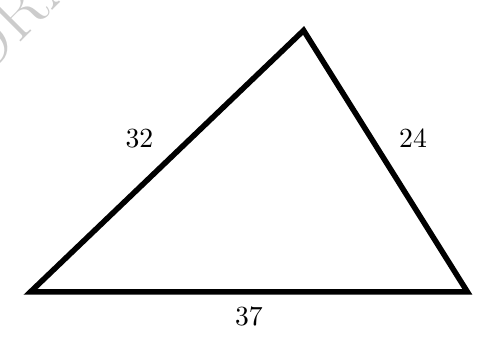
\begin{tikzpicture}[scale=.15]

	\coordinate (a) at (0,0);
	\coordinate (b) at (37,0);
	\coordinate (c) at (23.13,22.14);
	\draw[line width=2pt]  (a) -- (b) -- (c) -- cycle;
	
	\tkzLabelSegment[below = 2pt](a,b){$37$}
	\tkzLabelSegment[above left = 2pt](c,a){$32$}
	\tkzLabelSegment[above right = 2pt](b,c){$24$}

\end{tikzpicture}
\end{center}

\end{multicols}


\begin{tabular}{c || c}

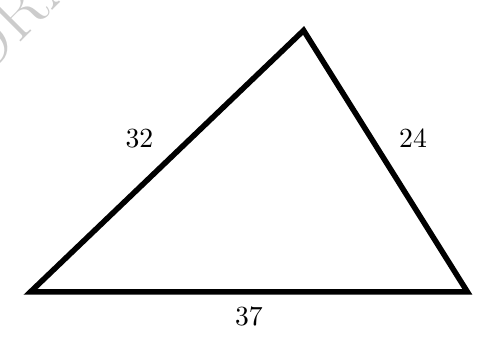
\begin{tikzpicture}[scale=.15]

	\coordinate (a) at (0,0);
	\coordinate (b) at (37,0);
	\coordinate (c) at (23.13,22.14);
	\draw[line width=2pt]  (a) -- (b) -- (c) -- cycle;
	
	\tkzLabelSegment[below = 2pt](a,b){$37$}
	\tkzLabelSegment[above left = 2pt](c,a){$32$}
	\tkzLabelSegment[above right = 2pt](b,c){$24$}
\end{tikzpicture}

&

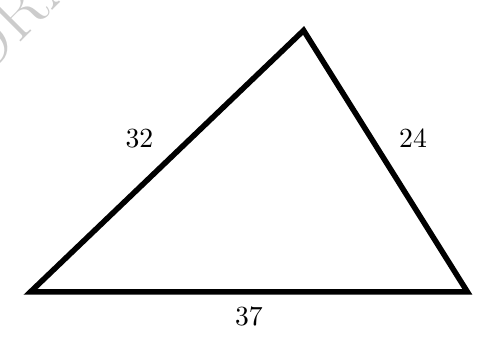
\begin{tikzpicture}[scale=.15]

	\coordinate (a) at (0,0);
	\coordinate (b) at (37,0);
	\coordinate (c) at (23.13,22.14);
	\draw[line width=2pt]  (a) -- (b) -- (c) -- cycle;
	
	\tkzLabelSegment[below = 2pt](a,b){$37$}
	\tkzLabelSegment[above left = 2pt](c,a){$32$}
	\tkzLabelSegment[above right = 2pt](b,c){$24$}
\end{tikzpicture}

\end{tabular}



\end{document}